\section{Nuestra herramienta: }

	En esta sección se explica como se llevó a cabo la implementación de la solución
	propuesta en la Sección \ref{Solucion}, cumpliendo a su vez el objetivo
	detallado en la Sección \ref{Objetivo}. Para ello se desarrollaron dos
	herramientas:
	\emph{Pure Objects Observable} (POO) para atacar a la problemática de la
	observabilidad, y \emph{Pure Object Transaction} (POT) para atacar a la
	problemática transaccional.
		
	\subsection{Selección de un framework de aspectos}  
		Un primer paso para la implementación de la herramienta fue la selección de una
		tecnología que permitiera desarrollar utilizando programación orientada a
		aspectos.
		Con ese objetivo, se evaluaron dos frameworks: Javassist
		\cite{chiba00loadtime} y AspectJ \cite{KiczalesHHKPG01}.
		
		\medskip 
		Encontramos que AspectJ es una herramienta de más alto nivel, que extiende
		el lenguaje Java agregando construcciones específicas para trabajar con
		los conceptos de la teoría de programación orientada a aspectos.
		Sin embargo, AspectJ requiere que el programador que use nuestro framework
		utilice un compilador específico, provisto por AspectJ. 
		Consideramos que esta característica es negativa, por condicionar el
		entorno de trabajo de los usuarios de nuestra herramienta.
		
		Javassist, por su lado, aplica los aspectos al momento de
		la carga de las clases, sólo requiere que utilicemos un \emph{ClassLoader}
		específico, resultando menos invasivo para los programadores de aplicaciones
		basadas en nuestra herramienta.
		Como aspecto negativo, notamos que es un framework de muy bajo nivel que
		carece de las abstracciones necesarias para modelar con aspectos y en cambio
		obliga a pensar a nivel de edición de expresiones en el bytecode de una clase
		compilada.
		
		Elegimos Javassist porque priorizamos minimizar el impacto hacia los usuarios
		de nuestra herramienta.
		Para minimizar los problemas asociados a utilizar un framework de tan bajo
		nivel, desarrollamos una herramienta que simplifica su uso agregando algunas
		abstracciones útiles. Esta herramienta se describe en la sección siguiente.

	\subsection{Desarrollo de Aspect for Pure Objects}
		El framework Javassist permite modificar directamente el \emph{bytecode} de
		una clase en el momento de cargarla.
		Por ser de tan bajo nivel es uno de los frameworks de aspecto más poderosos,
		pero a su vez el código que requiere es muy poco entendible.
		Por eso se desarrolló una herramienta llamada \emph{Aspect for Pure Objects} (APO), 
		que permite definir aspectos utilizando conceptos de más alto nivel y
		aplicárselo a un grupo de objetos. 
		
		La Figura \ref{aopImage} muestra esquemáticamente el diseño de la herramienta.
		Una instancia de \code{AdviceWeaver} se ocupa de aplicar los cambios sobre las
		clases.
		Cada uno de los cambios que debe realizar el \code{AdviceWeaver} está
		modelado por un \code{Advice}, que consiste de un \code{Predicate} y un
		\code{WeavingInstrumentor}.
		El \code{Predicate} tiene la responsabilidad de determinar el conjunto de
		clases sobre el que aplica el advice, mientras que el
		\code{WeavingInstrumentor} será el responsable de realizar las modificaciones
		sobre las clases seleccionadas.
		Finalmente una instancia de \code{APOClassLoader}, instalada como \emph{class
		loader} del sistema permite que antes de utilizar cualquier clase, esta pueda
		ser procesada por el \code{AdviceWeaver}.
		
		Para implementar las modificaciones se provee una implementación de
		\code{ExprEditor} que contiene una colección de modificaciones expresadas en un
		lenguaje de alto nivel y las traduce al lenguaje de bajo nivel que requiere el
		framework Javassist.
		La Figura \ref{pooCode} muestra un ejemplo de código de este lenguaje de alto nivel,
		tomado del framework POO, que se describe en la Sección \ref{poo}.
		
		\begin{figure}[h]
			\centering
			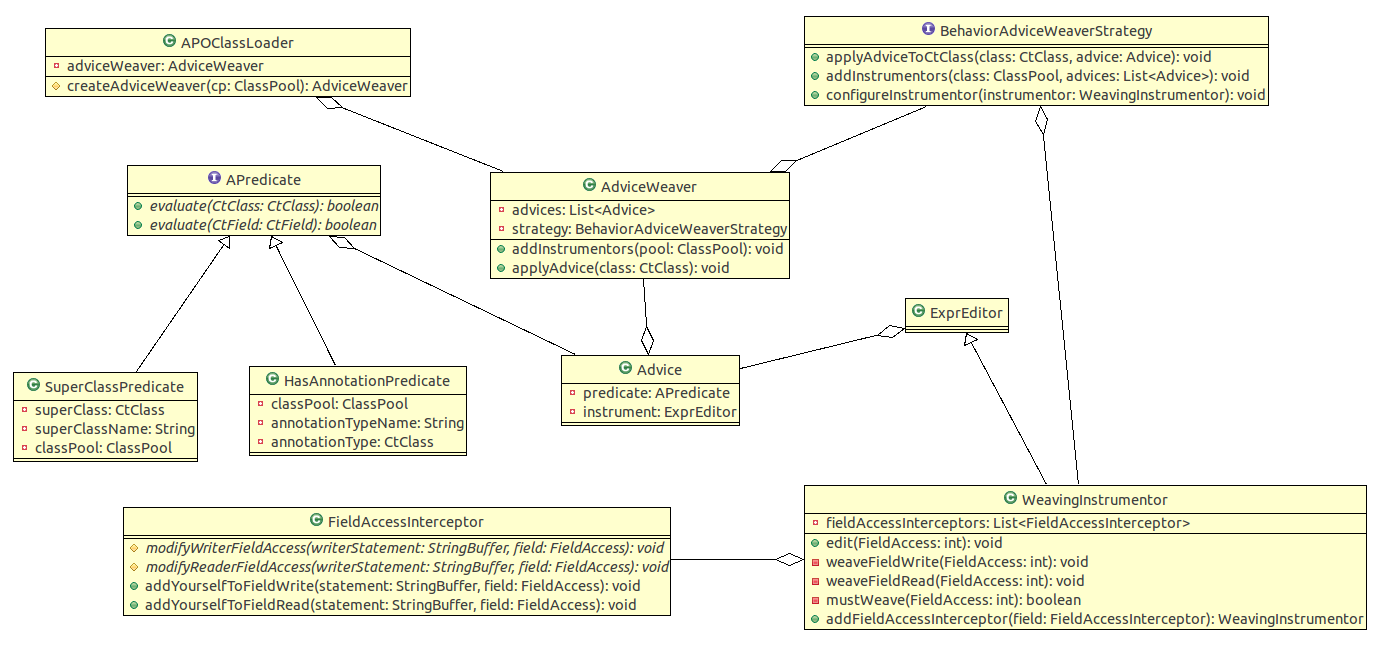
\includegraphics[width=450px, height=250px]{img/aop}
			\caption{Diagrama UML de la herramienta APO}
			\label{aopImage}
		\end{figure}	 
		
		
		A su vez, la Tabla \ref{table} describe las expresiones propias del lenguaje
		definido por APO, su traducción al lenguaje de expresiones de
		Javassist y su significado.
		
		\begin{figure}[h]
			\begin{lstlisting}
	$Object oldValue = $oldValue;
	$originalAsigment;
	$this.firePropertyChange('$fieldName', oldValue, $newValue);
			\end{lstlisting}
			\caption{Fragmento de código del framework POO}
			\label{pooCode}
		\end{figure}
		
		
		\begin{table*}[h]\centering
			\ra{1.3}
			\begin{tabular}{|+l^l^p{7cm}|}\toprule			
				\hline
				\rowstyle{\bfseries}%
					Expr. APO & Expr. Javassist & Significado \\
				\hline
					\$Object & java.lang.Object & El nombre completo de la clase Object \\
				\hline
					\$this & \$0 & El objeto receptor del mensaje.\\
				\hline
					\$newValue & \$1 & El primer parámetro del método. \\
				\hline
					\$oldValue &  \$0.getAtribute() & El valor del atributo antes de
				la asignación que está siendo modificada.\\
				\hline
					\$originalAsigment & \$0.atribute = \$1 & La asignación del atributo con el
				primer parámetro del método.\\
				\hline
					``\$fieldName'' & ``atribute'' & El nombre del atributo como un String.\\
				\hline
			\bottomrule
			\end{tabular} 
			\caption{Tabla de equivalencia de expresiones. ``atribute'' es el nombre del atributo propiamente dicho.}
			\label{table}
		\end{table*}
		
		APO es una herramienta abstracta, es decir, por si sola no modifica las clases, hay que configurarlo adecuadamente
		para optener el resultado deceado. POO y POT se contruyeron siguiendo esta filosofia de creacion de aspectos.
